%%%%%%%%%%%%%%%%%%%%%%%%%%%%%%%%%%%%%%%%%%%%%%%%%%%%%%%%%%%%%%%%%%%%%
%% Title: SOP LaTeX Template
%% Author: Soonho Kong / soonhok@cs.cmu.edu
%% Created: 2012-11-12
%%%%%%%%%%%%%%%%%%%%%%%%%%%%%%%%%%%%%%%%%%%%%%%%%%%%%%%%%%%%%%%%%%%%%

%%%%%%%%%%%%%%%%%%%%%%%%%%%%%%%%%%%%%%%%%%%%%%%%%%%%%%%%%%%%%%%%%%%%%
%%
%% Requirement:
%%     You need to have the `Adobe Caslon Pro` font family.
%%     For more information, please visit:
%%     http://store1.adobe.com/cfusion/store/html/index.cfm?store=OLS-US&event=displayFontPackage&code=1712
%%
%% How to Compile:
%%     $ xelatex main.tex
%%
%%%%%%%%%%%%%%%%%%%%%%%%%%%%%%%%%%%%%%%%%%%%%%%%%%%%%%%%%%%%%%%%%%%%%

\documentclass[letterpaper]{article}
\usepackage[letterpaper,margin=1.5in,nohe adfoot]{geometry}
\usepackage{fontspec, color, enumerate, sectsty}
\usepackage[normalem]{ulem}
\usepackage{natbib}
\usepackage{url}
\usepackage{todonotes}
\usepackage{setspace}
\usepackage{float}
\usepackage{xcolor}
\usepackage{listings}
\lstset{basicstyle=\ttfamily,
  showstringspaces=false,
  commentstyle=\color{red},
  keywordstyle=\color{blue}
}
\usepackage[htt]{hyphenat}
\definecolor{wildstrawberry}{rgb}{1.0, 0.26, 0.64}
\setlength\parindent{0pt}
\linespread{1.2}

%%%%%%%%%%%%%%%%%%%%%%%%%%%%%%%%%%%%%%%%%%%%%%%%%%%%%%%%%%%%%%%%%%%%%
%                      YOUR INFORMATION
%
%      PLEASE EDIT THE FOLLOWING LINES ACCORDINGLY!!
%%%%%%%%%%%%%%%%%%%%%%%%%%%%%%%%%%%%%%%%%%%%%%%%%%%%%%%%%%%%%%%%%%%%%
\newcommand{\soptitle}{Cyber Security Project Report}
\newcommand{\subtitle}{CSAW-HackML-2020}
\newcommand{\yourname}{Yang Li, Yuwen Liu, Xiaofeng Xu}
\newcommand{\youremail}{yl7014@nyu.edu, yl6927@nyu.edu, xx963@nyu.edu}

%% FONTS SETUP
\defaultfontfeatures{Mapping=tex-text}
\setromanfont[Path = fonts/, Ligatures={Common}]{adobe_caslon_pro}
\setmonofont[Path = fonts/, Scale=0.8]{monaco}
\setsansfont[Path = fonts/, Scale=0.9]{Optima-Regular}
\newcommand{\amper}{{\fontspec[Scale=.95]{Adobe Caslon Pro}\selectfont\itshape\&~{}}}
\usepackage[bookmarks, colorlinks, breaklinks,
pdftitle={\yourname - \soptitle}, pdfauthor={\yourname}, unicode, colorlinks=False, hidelinks]{hyperref}
\hypersetup{linkcolor=magneta,citecolor=magenta,filecolor=magenta,urlcolor=wildstrawberry}

%%%%%%%%%%%%%%%%%%%%%%%%%%%%%%%%%%%%%%%%%%%%%%%%%%%%%%%%%%%%%%%%%%%%%
%                      Title and Author Name
%%%%%%%%%%%%%%%%%%%%%%%%%%%%%%%%%%%%%%%%%%%%%%%%%%%%%%%%%%%%%%%%%%%%%
\begin{document}
\begin{center}{\huge \scshape \soptitle}\end{center}
\begin{center}{\large \subtitle}\end{center}
\begin{center}\vspace{0.2em} {\Large \yourname\\}
  {\youremail}\end{center}

%%%%%%%%%%%%%%%%%%%%%%%%%%%%%%%%%%%%%%%%%%%%%%%%%%%%%%%%%%%%%%%%%%%%%
%                      SOP Body
% NOTE: Use \amper instead of \&
%%%%%%%%%%%%%%%%%%%%%%%%%%%%%%%%%%%%%%%%%%%%%%%%%%%%%%%%%%%%%%%%%%%%%
\section*{Environment Setup}
Please see the \texttt{README} in the GitHub repository\footnotemark\footnotetext{\url{https://github.com/zjzsliyang/CSAW-HackML-2020}}. We introduce the dependencies as well as the bash commands to run the code.

\section*{Base Model Structure}
We implemented two approaches to detect and repair backdoored model. First is based on by \cite{wang2019neural} and second is based on \cite{gao2019strip}. These two approaches can can be divided into two parts, e.g. detecting the backdoor labels and repair the BadNets. Our models are based on the default model in the origin repo, as following Figure \ref{fig:base_structure} shows. 
\begin{figure}[H]
    \centering
    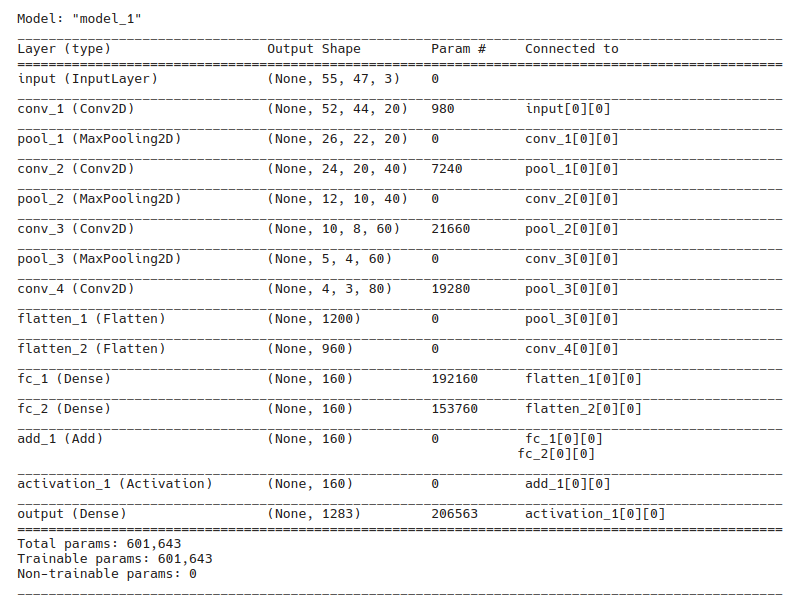
\includegraphics[width=10cm,  height=6cm]{img/model_structure.png}
    \caption{Model Structure}
    \label{fig:base_structure}
\end{figure}

\newpage
\section*{Neural Cleanse}
\subsection*{Detect Backdoors}
The key idea of Neural Cleanse\footnotemark\footnotetext{\url{https://sites.cs.ucsb.edu/~bolunwang/assets/docs/backdoor-sp19.pdf}} by  \cite{wang2019neural} is that if a model is poisoned, it requires much smaller modifications to cause the model to classify the wrong target label. So we decided to iterate all possible labels and check which one requires smaller modification to achieve the wrong result. The whole process will be divided into 3 steps:

\begin{enumerate}
    \item Find the minimal trigger. We try to find a trigger window with a fixed label. We assume this label is the target label of the attack backdoor trigger. The performance of this trigger depends on how small it is to misclassify all samples from other labels into the target label.
    
    \item Iterate the whole label sets. We run the loop for iterating all labels in the model, which is 1283 in our project. In other words, 1283 potential triggers will be created after this step.
    
    \item Choose the valid trigger. We need to choose the valid trigger in all 1283 triggers. It depends on the number of pixels the trigger trying to influence in the models. Our method is to calculate the L1 norms of all triggers. Then we will calculate the absolute deviation between all data points and the median. If the absolute deviation of a data point divided by that median is larger than 2, we mark it as a target trigger. The target trigger which is most effective to misclassify the model will be the ``reverse trigger'' we need to repair BadNets.
\end{enumerate}
The implementation of the step 1 and 2 is in the \href{https://github.com/zjzsliyang/CSAW-HackML-2020/blob/master/visualize_example.py}{\texttt{visualize\_example.py}} and \href{https://github.com/zjzsliyang/CSAW-HackML-2020/blob/master/visualizer.py}{\texttt{visualizer.py}}.

The implementation of the step 3 is in the \href{https://github.com/zjzsliyang/CSAW-HackML-2020/blob/master/mad_outlier_detection.py}{\texttt{mad\_outlier\_detection.py}}.

\subsection*{Repair BadNets}
In order to repair BadNets, we decided to patch the infected model by pruning the poisoned neurons in the BadNet with the ``reverse trigger''.

The target trigger poisoned neurons in the model to make it misclassify the label, so we need to find these neurons and set their output value to 0 so that the model will not be affected by the trigger anymore. 

Therefore we rank the neurons by differences between clean input and poisoned input produced by the 'reverse triggers'. We again target the second to last layer, and prune neurons by order of highest rank first. In order to keep the performance of the model on clean target, we decided to stop the iteration as soon as the model is not sensitive to the poisoned input any more.

You can find details in the \href{https://github.com/zjzsliyang/CSAW-HackML-2020/blob/master/repair_model.py}{\texttt{repair\_model.py}}.

\subsection*{Result \& Sample Output}
% [language=bash, caption={bash version}]
\begin{lstlisting}
#!/bin/bash
python3 repair_model.py sunglasses

base model in clean test: 97.77864380358535, poisoned: 99.99220576773187
pruned model in clean test: 86.83554169914264, poisoned: 1.161340607950117
repair model in clean test: 88.08261886204208, fixed poisoned: 100.0
elapsed time 1132.0141394138336 s
\end{lstlisting}

\noindent\rule{2cm}{0.4pt}
\begin{lstlisting}
python3 repair_model.py anonymous_1

base model in clean test: 97.1862821512081, poisoned: 91.3971161340608
pruned model in clean test: 95.12081060015588, poisoned: 3.0982073265783323
repair model in clean test: 79.81293842556508, fixed poisoned: 99.71745908028059
elapsed time 1085.563981294632 s
\end{lstlisting}

\noindent\rule{2cm}{0.4pt}
\begin{lstlisting}
python3 repair_model.py anonymous_2

base model in clean test: 95.96258768511302, poisoned: 0.0
pruned model in clean test: 96.18862042088854, poisoned: 0.03897116134060795
repair model in clean test: 78.95557287607171, fixed poisoned: 99.85385814497272
elapsed time 1077.5421595573425 s
\end{lstlisting}

\noindent\rule{2cm}{0.4pt}
\begin{lstlisting}
python3 repair_model.py multi_trigger_multi_target
base model in clean test: 96.00935307872174, poisoned: 30.452714990906728
pruned model in clean test: 95.86905689789556, poisoned: 1.575084437516238
repair model skipped.
elapsed time 1533.934408903122 s
\end{lstlisting}

% \begin{table}[H]\centering
% \begin{tabular}{|c|c|c|c|}
% \hline
% \textbf{methods} & \textbf{EEG} & \textbf{ECG-40} & \textbf{ECG-15} \\ \hline
% DTW              & 71.6         & 74.5            & 85.5            \\ \hline
% DWT              & 76.0         & 25.1            & 20.1            \\ \hline
% DFT              & 91.6         & 85.6            & 60.6            \\ \hline
% BoW              & 93.8         & 99.5            & 100             \\ \hline
% \end{tabular}
% \caption{Comparison of bag-of-words model}
% \label{table:res}
% \end{table}

% \section*{Concluding Remarks}


\bibliography{ref}
\bibliographystyle{chicago}
\end{document}